\vspace{-3cm}\chapter{The Basic Idea of Java OOP}

考虑到作业需要的是一份内容总结,而非讲义,故内容编排上和教学顺序有一定出入。

\section{0x00 基本概念}

重载(overload):作为一门现代化的语言,Java支持方法重载,即:只要方法名和参数类型不全相同即可视作一个新的方法。重载方法的原则遵循就近原则。

强制类型转换(cast):Java也支持变量强制类型转换,注意:这种转换只是一种对编译器的“欺骗”——即告诉编译器这一块为类型转换的目标类型。

Java中一切非原始类型的都以引用类型在程序中存在。

Java中每个引用变量有两个类型:
\begin{itemize}
    \item 静态类型:声明时定义的类型,在编译时确定并检查,也就是说cast改变的是那一块的静态类型。
    \item 动态类型:变量实际指向的类型,在运行时确定。
\end{itemize}

Java中用final关键字表示常量

\section{0x01 类}

Java中的一切函数(方法)、变量和代码都是在一个个类中。

自然而然地,由基本的面向对象思想,一个类可以被另一个类所继承,Java中用extends关键词。
\begin{lstlisting}[language = Java]
    public subClassA extends parentClassB{
        // ... 
    }
\end{lstlisting}

子类会继承父类的所有变量和方法,可以通过 super 调用形成独一无二的“is a”关系

每个类都有变量(Field)和函数(Method)两部分,类中成员的声明需要访问权限修饰符,修饰符主要在其他类调用该类中的成员时确认合法性,
Java中共有四种修饰符,各自含义如下:
\begin{table}[H]
    \centering
    \begin{tabular}{|c|c|c|c|c|}
        \hline
        \textbf{访问范围} & \textbf{private} & \textbf{friendly(默认)} & \textbf{protected} & \textbf{public} \\ \hline
        同一个类          & √                & √                     & √                  & √               \\ \hline
        同一个包中的其他类     & ×                & √                     & √                  & √               \\ \hline
        不同包中的子类       & ×                & ×                     & √                  & √               \\ \hline
        不同包中的非子类      & ×                & ×                     & ×                  & √               \\ \hline
    \end{tabular}
\end{table}


\subsection{abstract\& final}
abstract: 
\begin{itemize}
    \item abstract修饰的方法可以不定义,只能存在于abstract类中
    \item abstract修饰的类不能被直接实例化,类中可以存在非abstract方法
\end{itemize}

final: final修饰的类不能被继承,final修饰的方法也不能进行修改。


\section{0x02 接口}

由于Java只支持类对类的单继承,为了使继承更加地灵活,除了类,Java中还存在另一种和类相似的类型:接口。
接口需要定义方法,但不实现方法(不过随着Java版本的更新也有了default的方法实现)。

当一个类需要继承这个接口时,声明类时采用implements关键词,用法与extends类似。但一个类可以继承多个接口,接口与接口用逗号隔开。
\begin{lstlisting}[language = Java]
public subClassA extends parentClassB implements InterfaceA, InterfaceB{
    // ... 
}
\end{lstlisting}

如果一个类继承了某个接口,则它一定要实现接口中的所有方法。

类和接口不存在is a的关系。

考虑到接口可以独立作为一个类型,也可以被实现,后文的叙述中涉及继承的部分默认也适用于继承自接口。

\section{0x03 继承}

继承的思想很好理解和接受,但继承中存在大量细节需要说明和理解记忆。

\subsection{3.0 Constructor}

子类的构造方法的第一句必须是父类的构造方法,这一句也可以通过调用子类的其他构造方法以实现。

如果构造方法的第一句和上述不符,编译器会在第一句插一条父类的默认构造方法 super() ,如果父类没有默认的构造方法此处会编译报错。

\subsection{3.1 Override}

当子类中的某个\textbf{方法}和父类的方法名相同,修饰符访问范围更开放,且参数类型也相同时,我们称该方法覆盖(override)了父类中的原方法,
此时若想通过子类调用父类方法只能通过super()。

\subsubsection{override 流程}
\begin{enumerate}
    \item 当且仅当\textbf{方法}参数类型和方法名均相同时会被认为是override,开始检查override的合法性
    \item 当方法名和参数类型均相同,但返回值不同或访问权限更小,这个函数不合法,会出现编译错误
\end{enumerate}

\begin{figure}[H]
    \centering
    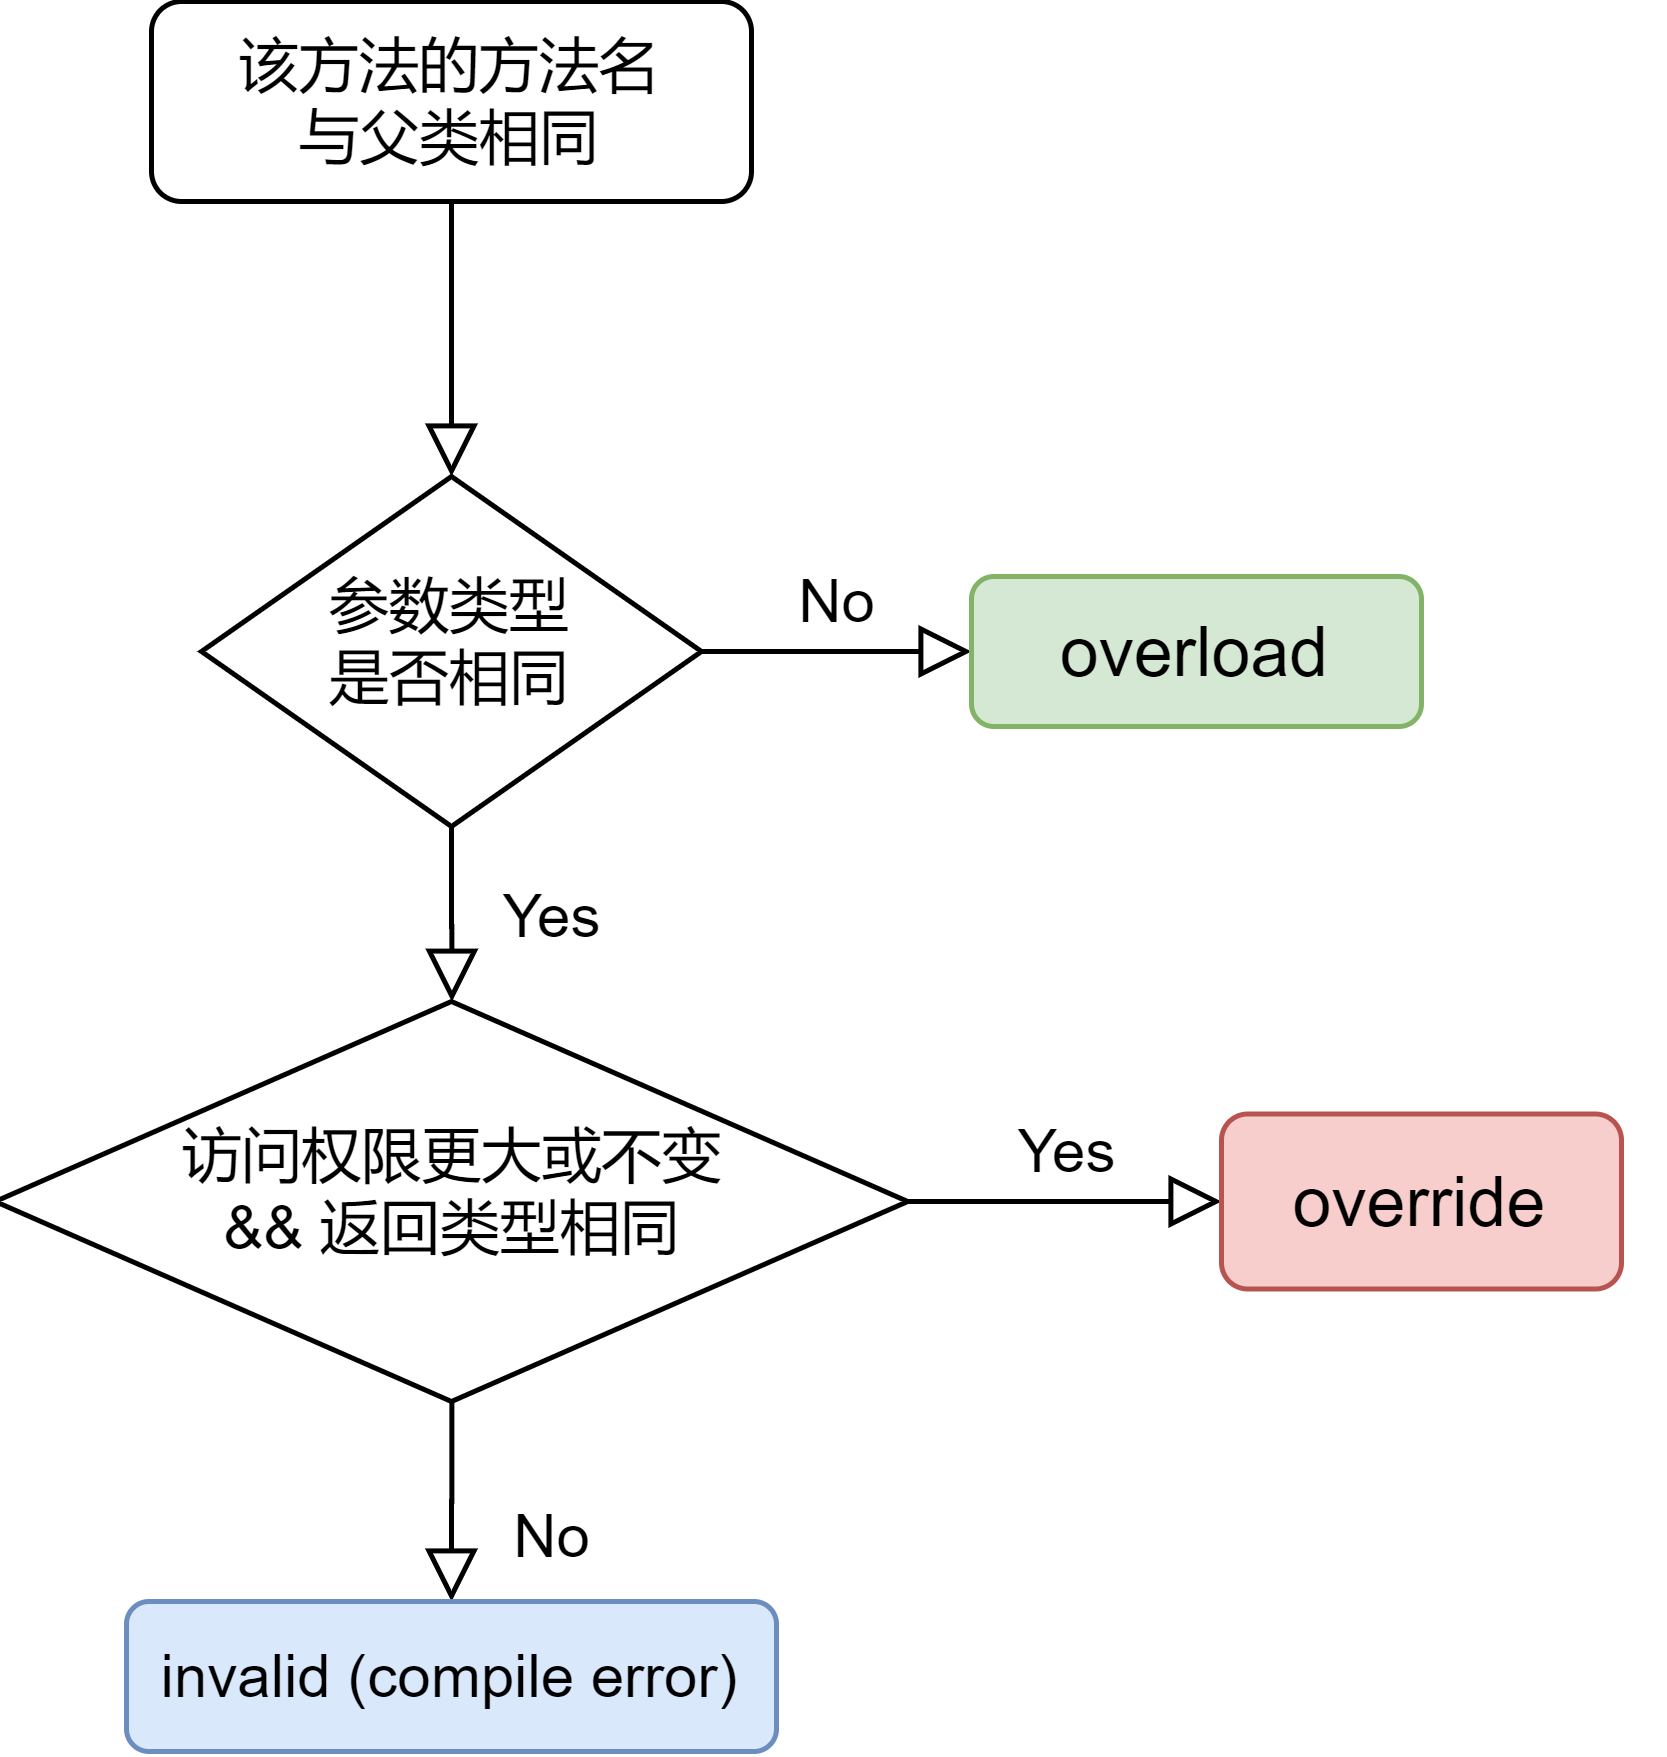
\includegraphics[width = 0.6\textwidth]{../pic/4/flowchart_override.png}
\end{figure}

\subsubsection{add \& override}

\textbf{\color{red}{变量中不存在覆盖的概念,如果变量出现重名,会新增一个变量。}}

如果出现重载,会新增一个方法。

\subsection{3.2 Check\& Selection}

从编译的角度看:在编译过程中需要检查程序中每一句的合法性,这时只能采用静态类型确认,对静态类型来说不合法就会报错。

\subsubsection{cast \& type}

有了继承的概念,我们可以先对cast的概念在继承的角度作进一步的说明。

编译时:当两个对象的类之间存在继承关系时可以cast,否则会出现compile error

运行时:如果对象的动态类型并非cast的结果,则会出现exception. 从继承关系上看,向上转换可以毫无顾忌地执行
(因为有“is a”关系),但向下转换时需要谨慎考虑。

\subsubsection{Variable field}

在java的类中,变量域依赖于静态类型而存在。

因此,如果需要不利用super访问父类的变量也可以利用cast转为父类再访问变量。

\subsubsection{Method}

除了实例方法外,类中的数据成员和类方法均依赖于对象的静态类型存在,也就是说在编译时就确定了要用哪个数据/方法。

实例方法比较特殊,采用一种动态选择的机制,在运行时才会依据引用变量指向的实例对象类型选择要执行的方法。

\section{0x04 Examples}

上述的概念尤其是3.2部分存在一定的抽象性,没有陷进坑里过很难一次性想明白,故提供几个样例程序如下

\lstinputlisting[language = Java, caption = {Bird.java}]{../../../ProblemSet/src/hw2/p4/Bird.java}

\lstinputlisting[language = Java, caption = {Dog.java}]{../../../ProblemSet/src/hw2/p4/Dog.java}

根据以上两个代码可以对下面这段代码有更好的理解
\lstinputlisting[language = Java, caption = {Supplier.java}]{../../../ProblemSet/src/hw2/p4/Supplier.java}

\section{0x05 Polymorphism}

什么是多态?

从程序到进程周期的角度看,Java中存在两种多态:

\begin{itemize}
    \item 静态多态(编译时多态性):同名方法可以有多个,在编译时能够确定执行同名方法中的哪一个,则称为编译时多态性.
    \item 动态多态(运行时多态):由于覆盖的影响,在编译时不能确定,只能在运行时才能确定执行多个同名方法中的哪一个,则称为运行时多态性.
\end{itemize}

从类的角度看,Java 中也存在类多态:

\begin{itemize}
    \item 方法重载:同一个类的同名方法可以重载;
    \item 子类重定义:子类可以重定义父类的成员,从而隐藏变量或者覆盖方法
\end{itemize}